\documentclass{beamer}

% This file is a solution template for:

% - Giving a talk on some subject.
% - The talk is between 15min and 45min long.
% - Style is ornate.



% Copyright 2004 by Till Tantau <tantau@users.sourceforge.net>.
%
% In principle, this file can be redistributed and/or modified under
% the terms of the GNU Public License, version 2.
%
% However, this file is supposed to be a template to be modified
% for your own needs. For this reason, if you use this file as a
% template and not specifically distribute it as part of a another
% package/program, I grant the extra permission to freely copy and
% modify this file as you see fit and even to delete this copyright
% notice. 


\mode<presentation>
{
  \usetheme[height=12mm]{Rochester}
  % or ...%

  \setbeamercovered{transparent}
%  % or whatever (possibly just delete it)
}


\usepackage[brazil]{babel}
% or whatever

% or whatever
%\usepackage{graphics}
\usepackage{times}
\usepackage[utf8]{inputenc}
\usepackage{url}

\newcommand{\nektar}{\ensuremath{\mathcal{N}\varepsilon \kappa \tau \alpha r}}
\newcommand{\ordem}[1]{ \ensuremath{\mathcal{O}[#1]}}
\newcommand{\pr}[1]{\ensuremath{ \mathbf{#1}}}    % \pr vem de preto
\newcommand{\etal}{\emph{et al.}}
\newcommand{\jac}[4]{ \ensuremath{ P_{#2}^{#3,#4}(#1) }}
\newcommand{\der}[2]{\ensuremath{ \frac{\partial #1}{\partial #2}}}
\newcommand{\convect}[2]{\ensuremath{ #1 \cdot \nabla #2}}
\newcommand{\R}{\ensuremath{ Re }}
\newcommand{\St}{\ensuremath{ St }}
\newcommand{\cpb}{\ensuremath{ C_{pb}}}
\newcommand{\transf}[3]{\ensuremath{ \int_{-\infty}^\infty #3\: e^{i #2 #1}\: d #2}}
\newcommand\clrms{\ensuremath{\sqrt{\overline{C_L^2}}}}
\newcommand{\epseudo}{\ensuremath{ \epsilon-\text{pseudospectro}}}
\newcommand{\lra}{\ensuremath{\longrightarrow}}

\newcommand{\wt}[1]{\ensuremath{\widetilde{#1}}}
\newcommand{\mcal}[1]{\ensuremath{\mathcal{#1}}}

\newcommand{\ol}[1]{\ensuremath{\overline{#1}}}
\newcommand{\us}{\ensuremath{u_*}}

\newcommand{\p}[1]{\ensuremath{ \mathbf{#1}}}    % \pr vem de preto
\newcommand{\qrq}{\ensuremath{\quad\lra\quad}}
\newcommand{\qqrq}{\ensuremath{\qquad\lra\qquad}}
\newcommand{\pd}{\ensuremath{\partial}}
\newcommand{\bigO}[1]{\ensuremath{\mathcal{O}\left(#1\right)}}


\title{Modelos, Escalas e Semelhança}


\author{Paulo Jabardo}

\titlegraphic{
\includegraphics[width=4cm]{figuras/logo-ipt.png}}%}
%   \includegraphics[width=2cm]{fig
%}
\date{17-11-2023}





\begin{document}
\maketitle

\begin{frame}{Apresentação}

  \begin{itemize}
  \item Análise dimensional
  \item Por que não o nome tradicional???
  \item Qual a fixação com mecânica dos fluidos?
  \item Porque agora?
  \end{itemize}
\end{frame}  

\begin{frame}{Estrutura}
  \begin{itemize}
  \item Modelos e escalas
  \item Invariância e simetria
  \item Sabemos bastante: geometria e equações diferenciais
  \item Conseguimos simplificar bastante
  \item Análise dimensional
    \begin{itemize}
    \item As leis físicas não podem depender do sistema de unidades
    \item Dimensões e unidades
    \item Porque as unidades são sempre monômios?
    \item Teorema dos $\Pi$s de Buckingham
    \item Semelhança e simplificação
    \end{itemize}
  \item Exemplos
  \end{itemize}
\end{frame}  

\begin{frame}{O que cai mais rápido? Uma bola de boliche ou uma pena?}

Quem está respondendo?
\begin{itemize}
 \item Estudante que acabou de fazer o vestibular
 \item Uma criança de 5 anos
\end{itemize}
 
Que tal fazer um experimento?

\end{frame}  

\begin{frame}{Observações sobre os experimentos}
  \begin{itemize}
  \item Pena - Extremamente complexo quando cai no ar
  \item Penas - Também é complexo quando cai no vácuo (logo no comecinho)
  \item O ar tem efeito pequeno na bola de boliche
  \item O gatilho tem uma dinâmica complicadíssima
    \begin{itemize}
    \item Elasticidade do sistema
    \item Atrito da argola
    \item dinâmica do cabo que segura a bola
    \end{itemize}
  \end{itemize}
\end{frame}  

\begin{frame}{Algumas escalas do sistema}
  \begin{itemize}
  \item Peso da bola de boliche
  \item $t_{gatilho}$ - Escala de tempo para começar cair
  \item Geometria: diâmetro, área, volume, rugosidade esfericidade, etc
  \item outros...
  \end{itemize}
\end{frame}

\begin{frame}{Velocidade terminal da bola}
\[
ma = mg - F_a
\]

\[
F_a = C_D \times A \times \frac{1}{2}\rho U^2
\]

\[
ma = 0  \: \longrightarrow \: F_a = mg \: \longrightarrow \: U_{terminal} = \sqrt{\frac{2 m g}{C_D A \rho}}
\]

Chegamos na equação diferencial

\[m \frac{d^2 z}{dt^2} = -mg + C_D A \frac{1}{2} \rho \left(\frac{dz}{dt}\right)^2\]


\end{frame}
  

\begin{frame}{Mase e uma bexiga de hélio?}
Temos que adicionar o empuxo!

\[m \frac{d^2 z}{dt^2} = -mg + \frac{\pi \rho g D^3}{6} + C_D \frac{\pi D^2}{4} \frac{1}{2} \rho \frac{dz}{dt}\left|\frac{dz}{dt}\right|\]

Será que esse modelo é completo?
\begin{itemize}
\item Claramente não no caso geral
\item Talvez para um corpo rígido? Mais ou menos...
\item Se quiser tratar o problema completo, você vai ficar louco!!!
\end{itemize}
\end{frame}

\begin{frame}{Qualquer (?) problema físico}
  \[X_1 + X_2 + \cdots + X_n = 0\]

  Modelo
  \begin{itemize}
    \item Equação (ou equações)
    \item Aproximações de $X_i$
    \item $|X_k| \ll |X_i|$ posso desprezar $X_k$ ou pelo menos usar um modelo simples
    \item Se um termo cresce, os outros precisam diminuir...
  \end{itemize}

\end{frame}


\begin{frame}{Um outro problema simples}

  \begin{itemize}
   \item Fluxo de ar constante 
   \item Passando por um aquecedor elétrico com potência constante
   \item Termino o experimento
   \item \textbf{Desligo o aquecedor}
   \item Aumento a vazão de ar
   \item O que acontece com a temperatura do ar de saída?
  \end{itemize}
\end{frame}

\begin{frame}{Frases que definem bem a modelagem}

 L. Tolstói  \begin{quote}
    Famílias felizes são felizes da mesma maneira, famílias infelizes são miseráveis cada um de um jeito único.
  \end{quote}

 H. L. Mencken (Scopes Monkey trial)
 \begin{quote}
Todo problema complexo tem uma solução simples, elegante e errada.
  \end{quote}
  
Ditados populares
  \begin{quote}
    Más vale malo conocido que bueno por conocer.
  \end{quote}

  \begin{quote}
    Más sabe el diablo por viejo que por diablo
  \end{quote}
  
\end{frame}


\begin{frame}{Modelos físicos X modelos matemáticos}
  \begin{itemize}
  \item Não farei distinções!
  \item Em sentido abstrato as dificuldades são as mesmas
  \item Em um modelo matemático, fixou as equações fixou o modelo
  \item Em um mdelo físico, fixou as condições de laboratório, fixou o modelo
  \item Fácil "fixar" a física em um modelo matemático
  \item Alguns problemas físicos intratáveis matematicamente são "simples" no laboratório
  \end{itemize}
\end{frame}

\begin{frame}{Um pouco de geometria}
\centering
\begin{tabular}{|c|c|c|c|}
  \hline
  Geometria & 
    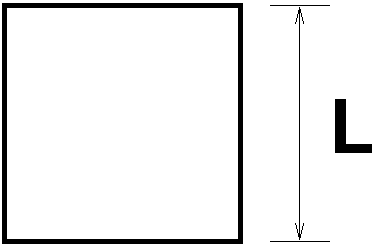
\includegraphics[width=0.25\textwidth]{./figuras/quadrado.pdf} & 
    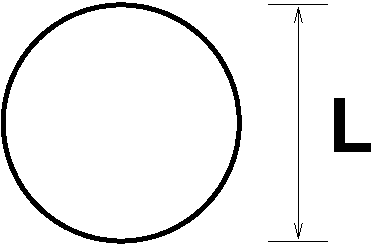
\includegraphics[width=0.25\textwidth]{./figuras/circulo.pdf} & 
    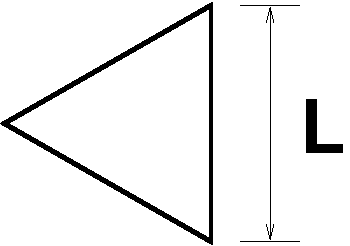
\includegraphics[width=0.25\textwidth]{./figuras/triangulo.pdf}\\
    \hline
    Área & $L^2$ & $\pi D^2/4$ & $\sqrt{3}/4 L^2$ \\
    \hline
    Perímetro & $4L$ & $\pi D$ & $3L$ \\
    \hline
\end{tabular}

    \[ A \sim L^2 \]

    \[ P \sim L \]
    
\[
\frac{A}{L^2} = k_1 \qqrq \frac{P}{L} = k_2
\]

\end{frame}

\begin{frame}{Isso vale mesmo para geometrias mais ``complexas''}
  \begin{center}
    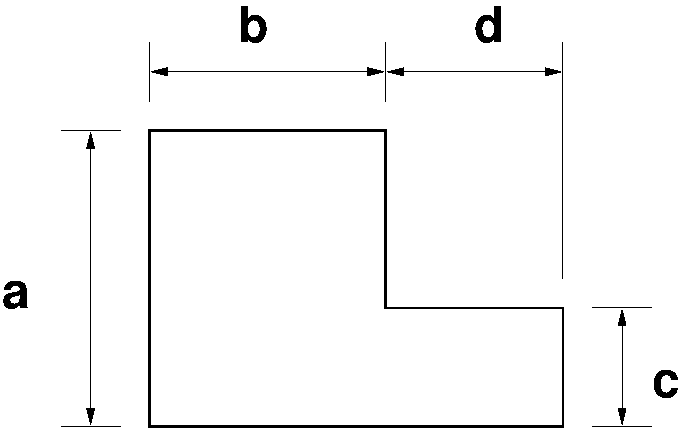
\includegraphics[width=0.5\textwidth]{./figuras/L2d.pdf}
  \end{center}
  Area: $A = a\cdot b + c\cdot d$, perímetro: $P = a + 2b + 2d + c$.

  \[
b = \alpha_1\cdot a, \qquad d = \alpha_2\cdot a, \qquad c = \alpha_3\cdot a
\]
A área e o perímetro desta figura geométrica são dadas por:
\[
\frac{A}{a^2} = (\alpha_1 + \alpha_2\cdot\alpha_3) \qquad \frac{P}{a} = (1 + 2\alpha_1+2\alpha_2+\alpha_3)
\]
\end{frame}

\begin{frame}{Floco de Koch}
\centering
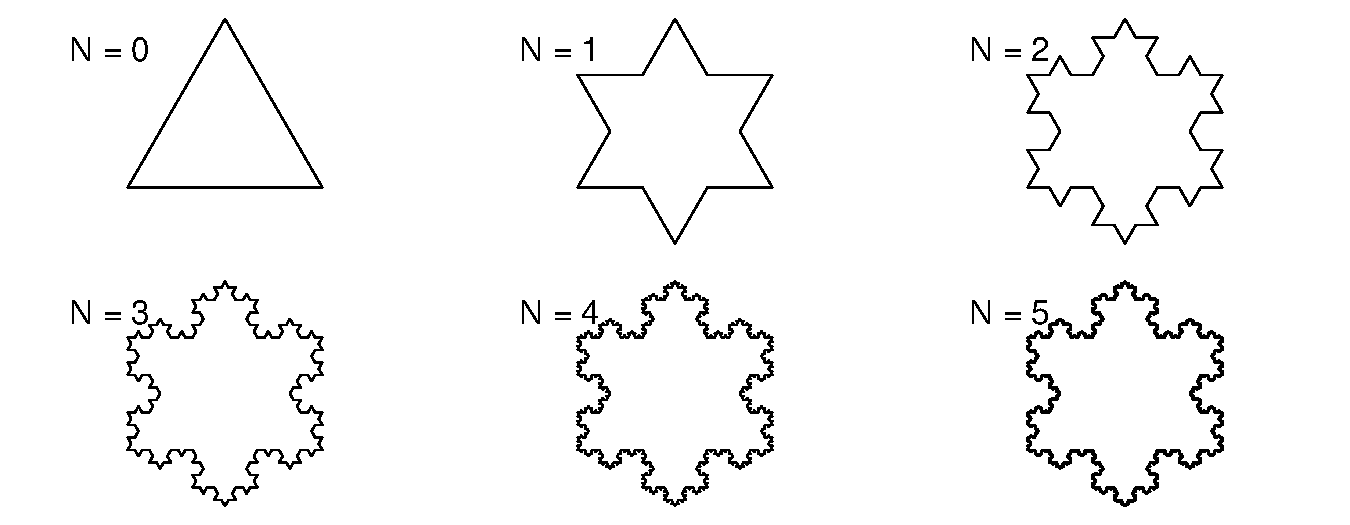
\includegraphics[width=\textwidth]{./figuras/koch.pdf}

\[
\frac{A}{L^2} = \frac{\sqrt{3}}{20} \cdot \left[8 - 3\left(\frac{4}{9}\right)^N\right] \qrq \frac{P}{L} = 3\cdot\left(\frac{4}{3}\right)^N
\]
\end{frame}


\begin{frame}{Floco de Koch - Autossemelhança}
  \centering
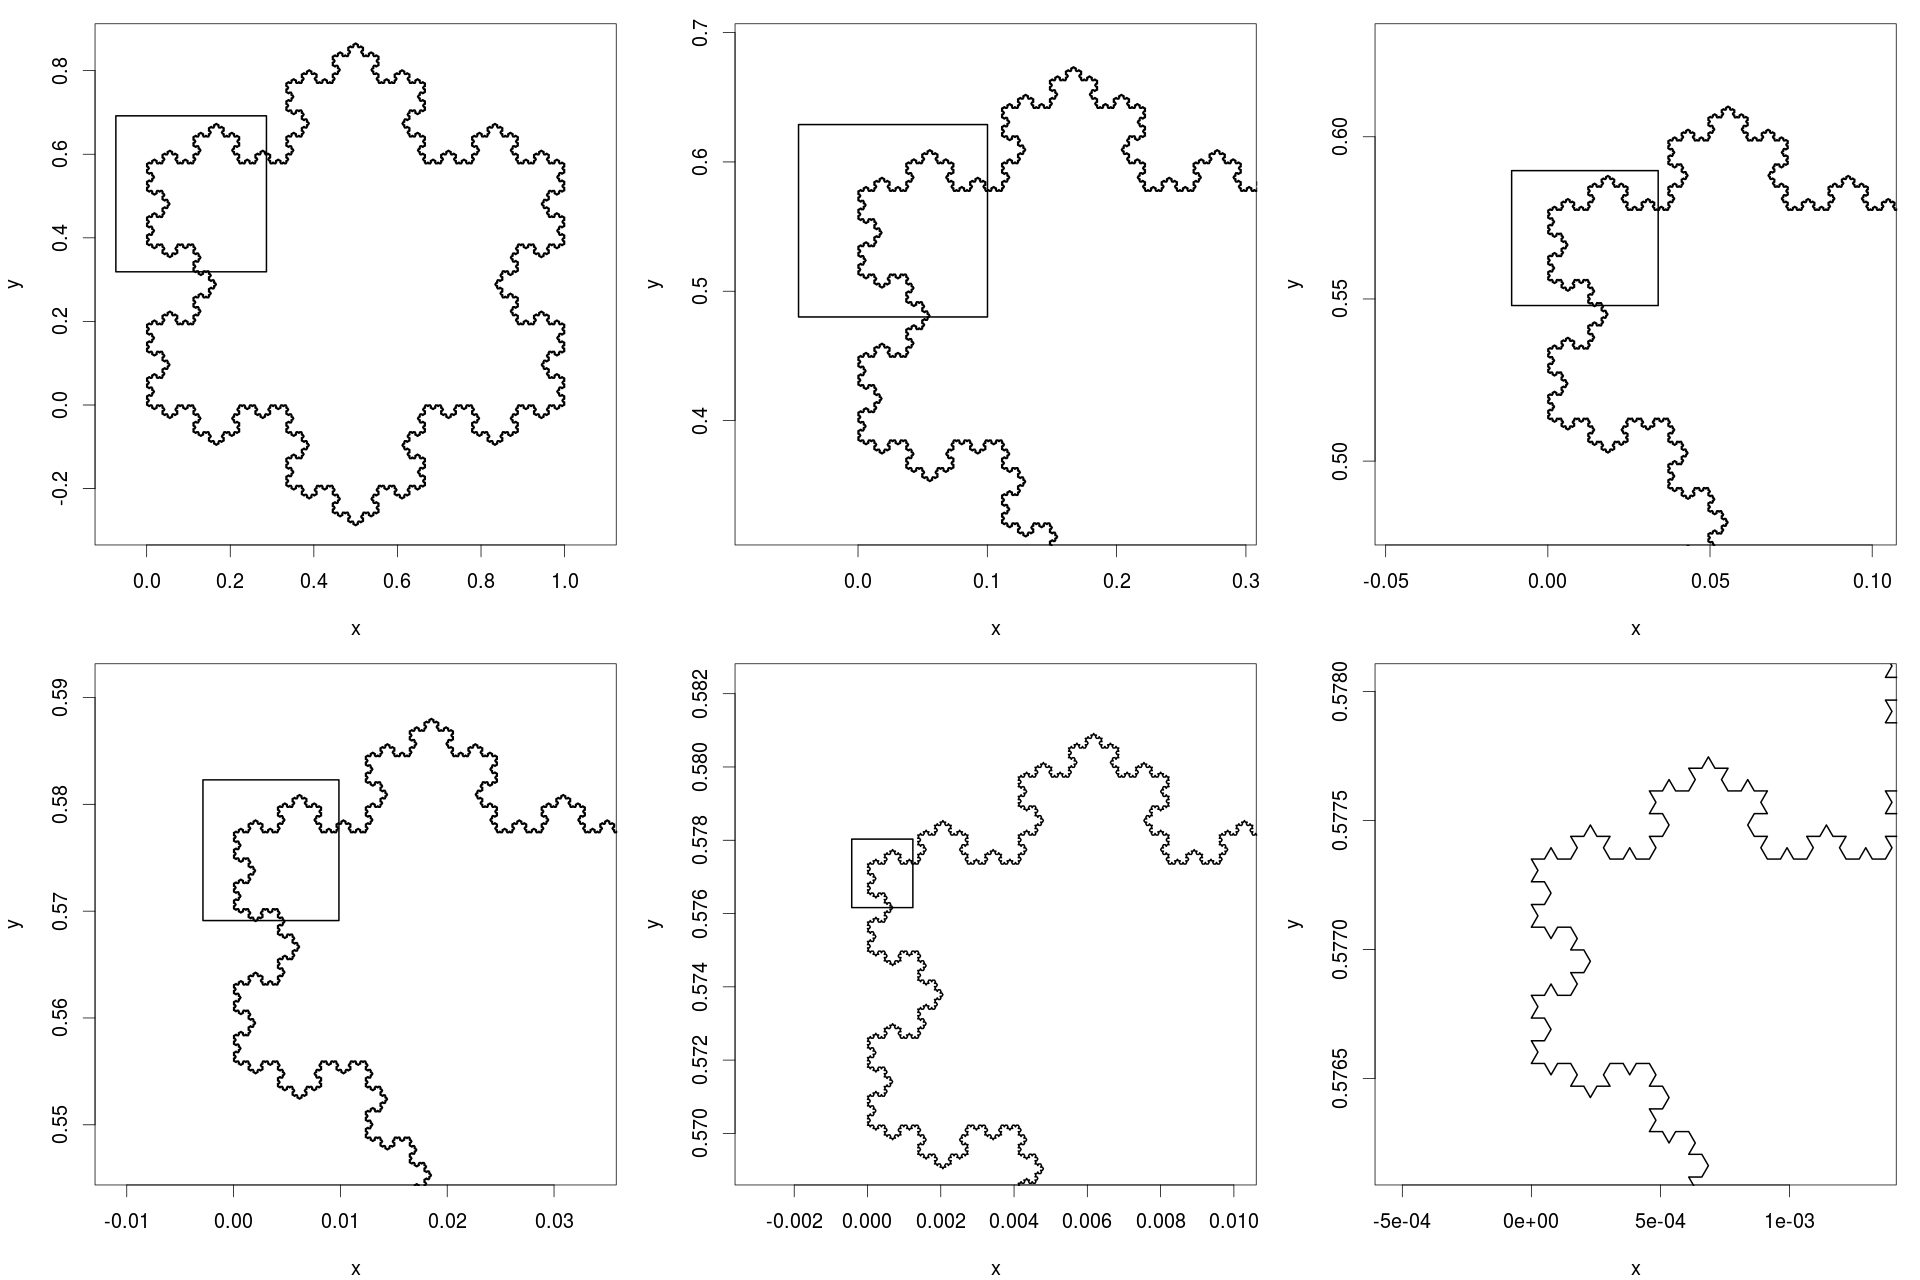
\includegraphics[width=1\textwidth]{./figuras/koch-self.png}
\end{frame}

\begin{frame}{Leis de potência - Autossemelhança}
  \centering
  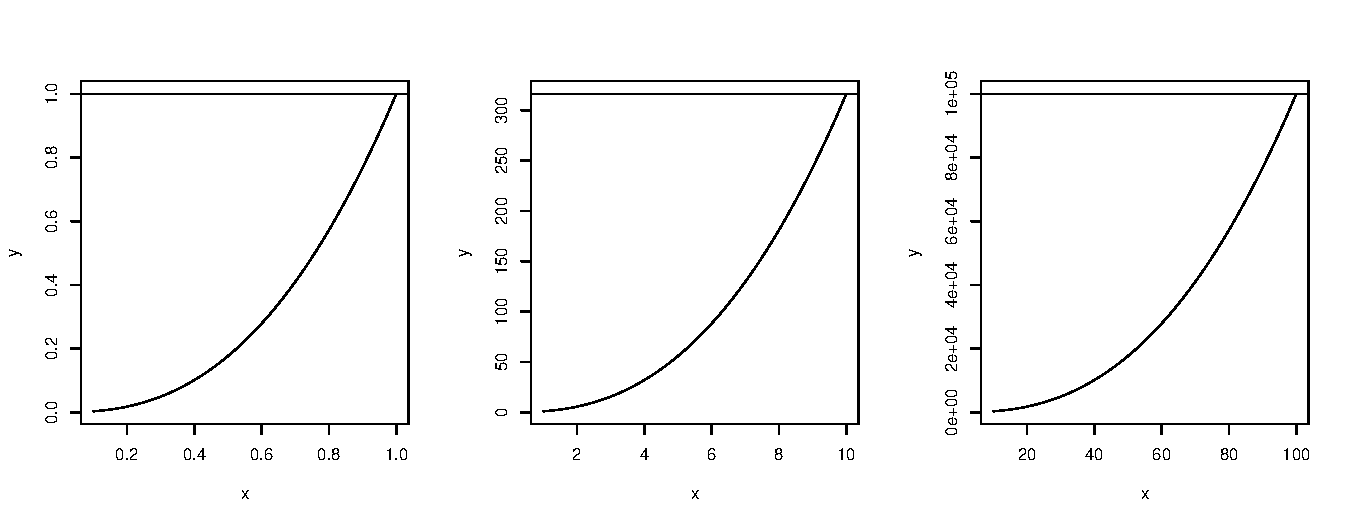
\includegraphics[width=\textwidth]{./figuras/power.pdf}
\end{frame}


\begin{frame}{Teorema de Pitágoras}
  \centering
  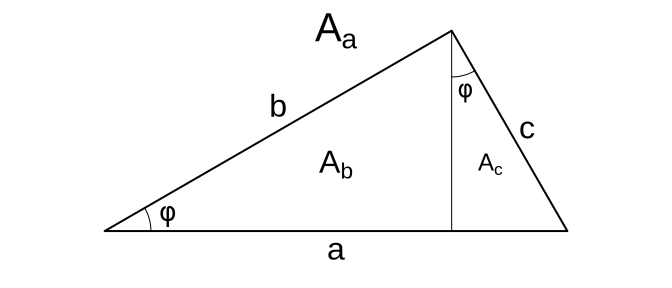
\includegraphics[width=0.9\textwidth]{./figuras/pitagoras}
  
\[
A(h,\phi) = h^2\cdot f(\phi)
\]
\[
A_a a^2\cdot f(\phi) = A_b + A_c = b^2\cdot f(\phi) + c^2\cdot f(\phi)
\]
\[
a^2 = b^2 + c^2
\]
\end{frame}

\begin{frame}{Nós sabemos muito!}
  \begin{itemize}
  \item Ninguém aqui vai ganhar premio Nobel!
  \item A física básica já é conhecida!
  \item Mas ainda não sabemos de todas as suas nuances
  \item Um problema só é ``tratável'' se simplificarmos
  \item Ciência é reducionista
  \item O mais  importante é saber o que desprezar!
  \end{itemize}
\end{frame}

\begin{frame}{Pendulo simples}
  \centering
  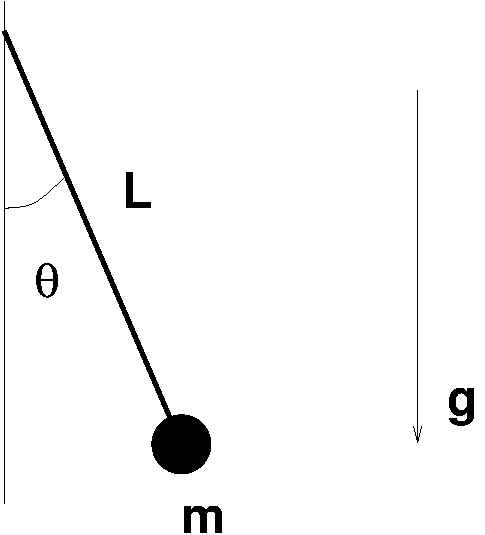
\includegraphics[width=0.3\textwidth]{./figuras/pendulo.pdf}
\end{frame}

\begin{frame}{Redução do modelo}
  \begin{itemize}
  \item Vamos desprezar radiação solar
  \item Vamos desprezar a variação de $\p{g}$
  \item Vamos desprezar a força de Coriolis
  \item O fio é perfeitamente rígido e sem massa e diâmetro nulo
  \item Vamos desprezar o atrito
  \item outros e mais outros...
  \end{itemize}
\end{frame}


\begin{frame}{Redução do modelo}
  Esfera de aço de 1cm, L=1 m, velocidade de 1 m/s

  
  \centering
  \begin{tabular}{c|c|c}
    \hline
    Força & Expressão & \% gravidade \\
    \hline
   Gravidade & $F_g = mg$ &   0.04 N\\
   Atrito &  $F_a = C_D 1/2 \rho_a  U^2 A$ &  $0.1$\% \\
   Coriolis & $F_c = 2m\Omega\sin\phi$  & $6\times 10^{-4}$ \% \\
   Radiação solar &  $10\mu N/m^2 \times A$ & $2\times 10^{-6}$ \%\\
   \hline
  \end{tabular}
\end{frame}
  
\begin{frame}{Modelo matemático simples}
\[
m\cdot L^2\cdot\frac{d^2\theta}{dt^2} + m\cdot g\cdot L\cdot \sin\theta = 0
\]

com as seguintes condições de contorno:
\[
t = 0 \qrq \theta=\theta_0, \quad\frac{d\theta}{dt} = 0
\]
\[
\frac{L}{g}\frac{d^2\theta}{dt^2} + \sin\theta = 0 
\]

\end{frame}


\begin{frame}{Escolher a régua certa}
  \[
  t_* = \frac{t}{t_0}\qrq \quad\text{onde}\quad t_0 = \sqrt{\frac{L}{g}}
\]
chega-se à equação adimensional
\[
\frac{d^2\theta}{dt_*^2} + \sin\theta = 0 
\]

\end{frame}

\begin{frame}{Período de oscilação}
  Para $\theta_0$ pequeno, $\sin\theta \approx \theta$
  \[
  T = 2\pi\sqrt{\frac{L}{g}}
  \]
  Em geral, temos:
\[
T = 2\pi\sqrt{\frac{L}{g}}\cdot\varphi(\theta_0)   
\]
\end{frame}


\begin{frame}{Difusão de calor em uma barra}
  \[u = u(x,t) \]
  
\[
\frac{\pd u}{\pd t} = \alpha \frac{\pd^2 u}{\pd x^2}
\]
Condições de contorno e iniciais
\begin{itemize}
\item $u(x,0) = 0$
\item $u(0,t) = 0$, $u(L,t) = u_0$
\end{itemize}

Solução para $t\longrightarrow\infty$,
\[
\lim_{t\to\infty} {u(x,t)} = \frac{x}{L} u_0
\]

\end{frame}

\begin{frame}{Barra infinita: autosemelhança}
  \[L\to\infty\]
  Qual a escala de comprimento??? Tem que sair do próprio problema!

\[
\frac{t\alpha}{L_0^2} = cte\lra L_0 = \sqrt{t\alpha} \lra \eta = \frac{x}{L_0} \lra \frac{u}{u_0} = f(\eta)
\]
Mas $\eta$ é uma escala que varia com o tempo!

\end{frame}

\begin{frame}{Solução da barra infinita}
  Substituindo $u/u_0 = f(\eta)$:
  \[
f''(\eta) + \frac{\eta}{2} f'(\eta) = 0
\]

com $f(0) = 0 \qquad\qquad \lim_{\eta\to\infty} f(\eta) = 1$

Assim, chegamos à solução do problema:

\[
f(\eta) = \mathrm{erf}\left(\frac{\eta}{2}\right)
\]

\end{frame}


\begin{frame}{Escoamento ao redor de uma esfera}

  \[
  \frac{\pd\p{u}}{\pd t} + \p{u}\cdot\nabla\p{u} = -\frac{1}{\rho}\nabla p + \nu\nabla^2\p{u} \qquad\qquad \nabla\cdot\p{u} = 0
  \]
  \[
 r\lra\infty \quad \p{u}\lra U_0\p{\hat{i}} \qquad\qquad r=\frac{D}{2}\quad \p{u} = \p{0}
\]

Hipóteses:
\begin{itemize}
\item Mecânica do contínuo
\item Fluido incompressível
\item Propriedades constantes
\end{itemize}
\end{frame}



\begin{frame}{Vamos usar uma régua adequada}
\[
\begin{aligned}
&x_* = \frac{x}{D}, \quad y_* = \frac{y}{D}, \quad z_* = \frac{z}{D}\\
&\p{u}_* = \frac{\p{u}}{U_0}, \quad p_* = \frac{p}{P_0}, \quad t_* = \frac{t}{t_0} = \frac{tU_0}{D} \\
\end{aligned}
\]
Chegamos à seguinte equação diferencial:
\[
\frac{\pd\p{u}_*}{\pd t_*} + \p{u}_*\cdot\nabla_*\p{u_*} = -\frac{P_0}{\rho U_0^2}\nabla_* p_* + \frac{1}{Re}\nabla_*^2\p{u}_* \qquad \nabla_*\cdot\p{u}_* = 0
\]

e as condições de contorno são:
\[
 r_*\lra\infty \quad \p{u}_*\lra \p{\hat{i}} \qquad\qquad r_*=\frac{1}{2}, \p{u}_* = \p{0}
\]

\end{frame}

\begin{frame}{O que ganhamos com isso?}
  Originalmente,
  \[
u = f(t, x, y, z, U_0, D, \mu, \rho), \qquad F_A =  F_A(t,U_0, D, \mu, U_0)
\]
Agora temos
\[
u = U_0 \varphi\left(\frac{t U_0}{D}, \frac{x}{D}, \frac{y}{D}, \frac{z}{D}, \frac{\rho U_0 D}{\mu}\right), \qquad C_D = \frac{F_A}{\rho U_0^2 D^2} = C_D\left( \frac{\rho U_0 D}{\mu}\right)
\]



\end{frame}


\begin{frame}{Equações de Euler - $Re\lra\infty$}
  Se $Re$ é muito grande e admitimos regime permanente,
  \[
  \p{u}_*\cdot\nabla_*\p{u_*} = -\frac{P_0}{\rho U_0^2}\nabla_* p_* %\qqrq P_0\sim\rho U_0^2
  \]

  Agora, conseguimos chegar a uma escala de pressão:

  \[
P_0 = \rho U_0^2
\]
\end{frame}

\begin{frame}{E se a velocidade ao longe varia?}
  \[
U_\infty = U_0\cdot\left(1 + \epsilon_0\cdot\cos \omega_0 t\right)
\]

Com isso chegamos a
\[
\Omega\frac{\pd\p{u}_*}{\pd t_*} + \p{u}_*\cdot\nabla_*\p{u_*} = -\frac{P_0}{\rho U_0^2}\nabla_* p_* + \frac{1}{Re}\nabla_*^2\p{u}_*  \qquad \Omega = \frac{D\omega_0}{U_0}
\]
Originalmente tínhamos a escala de tempo $t_0 = D/U_0$ agora temos uma nova escala $t_1 = 1/\omega_0$.

Um novo adimensional:
\[
\Omega = \frac{t_1}{t_0} = \frac{D\omega_0}{U_0}
\]

E se a variação for mais complicada? (turbulência por exemplo)
\end{frame}

\begin{frame}{Complicando o problema: vibração da esfera}
  Uma nova equação:
  \[
y''(t) + 2\zeta\omega_Ny'(t) + \omega_N^2y(t) = \frac{F_{fluido}(t)}{m}
\]
Vamos usar a escalas de comprimento $D$ e tempo $t_0 = D/U_0$:
\[
\frac{d^2y_*}{dt_*^2} + 2\frac{\zeta}{V_R} \frac{dy_*}{dt_*} + \frac{1}{V_R^2} y_* = \frac{\rho D^3}{m} \cdot \varphi\left(t_*\right)
\]

$F_{fluido}(t) = \rho U_0^2 \times D^2 \varphi(t_*)$

Novos adimensionais

\[
\frac{\rho D^3}{m}  \qquad V_R = \frac{t_2}{t_0} = \frac{U_0}{\omega_N \cdot D} \qquad \frac{1}{t_2} = \omega_N = \sqrt{\frac{k}{m}}
\]



\end{frame}


\begin{frame}{E usando a escala de tempo do oscilador no escoamento?}
  Invertemos o problema!
\[
\frac{1}{V_R}\frac{\pd\p{u}_*}{\pd t_*} + \p{u}_*\cdot\nabla_*\p{u_*} = -\frac{P_0}{\rho U_0^2}\nabla_* p_* + \frac{1}{Re}\nabla_*^2\p{u}_* 
\]
\[
\frac{d^2y_*}{dt_*^2} + 2\zeta\frac{dy_*}{dt_*} + y_* = \frac{\rho D^3}{m} \cdot V_R^2 \cdot \varphi_1\left(t_*\right)
\]

O problema é o mesmo!
\end{frame}


\begin{frame}{Semelhança}

  Parâmetros adimensionais:
  \begin{itemize}
  \item Aparecem na adimensionalização das equações
  \item Fixando estes adimensionais, temos famílias de soluções
  \item Semelhança: soluções com parâmetros diferentes de mas da mesma família
\end{itemize}
  
\end{frame}

\begin{frame}{Processo simplificado}
  \begin{itemize}
  \item Adimensionalizar dá trabalho
  \item As equações diferenciais são leis físicas simples
  \item Podemos aplicar estas leis simples diretamente a estimativas
\end{itemize}
  
\end{frame}
\begin{frame}{Exemplo: esfera na base elástica}

  Forças agindo na esfera:
  \begin{itemize}
  \item Força elástica: $\bigO{k\cdot D}$
  \item Inércia da esfera: $\bigO{ma} \sim \bigO{m\cdot D/t_0^2} = \bigO{mU_0^2/D}$
  \item Força do fluido - viscosa: $\mu\partial U / \partial y A \sim \mu U_0 D$
  \item Força do fluido - forças de pressão: $\bigO{\rho U^2 D^2}$
  \end{itemize}
  
  Balanço das forças
  \[
  \sum F_i = ma \lra \bigO{m U_0^2 / D} = \bigO{k D}  + \bigO{\mu U_0 D} + \bigO{\rho U^2 D^2}
  \]
  A idéia é compara os diferentes termos. Então dividimos cada termo por um dos termos.
\end{frame}
\begin{frame}{Dividindo a equação por um dos termos}
  \begin{itemize}
  \item $\rho U_0^2 D^2$
    \[
    \bigO{\frac{m}{\rho D^3}}  = \bigO{\frac{k}{\rho U_0^2 D}}+  \bigO{\frac{\mu}{\rho U_0 D}} + \bigO{1}
    \]
  \item $mU_0^2/D$
    \[
\bigO{1} = \bigO{\frac{\omega_N^2 D^2}{U_0^2}} + \bigO{\frac{\rho D^3}{m}} + \bigO{\frac{\mu D^2}{m U_0}}
\]
\end{itemize}
\end{frame}

\begin{frame}{Semelhança (2)}

  \begin{itemize}
  \item Diferentes adimensionais: $\Pi = \Pi\left(\Pi_1, \Pi_2, \ldots, \Pi_N\right)$
  \item Modelo e protótipo
  \item $\left(\Pi_k\right)_m = \left(\Pi_k\right)_p$
  \end{itemize}

  
\end{frame}

\begin{frame}{Desafio: Camada limite laminar e solução de Blasius}
\centering
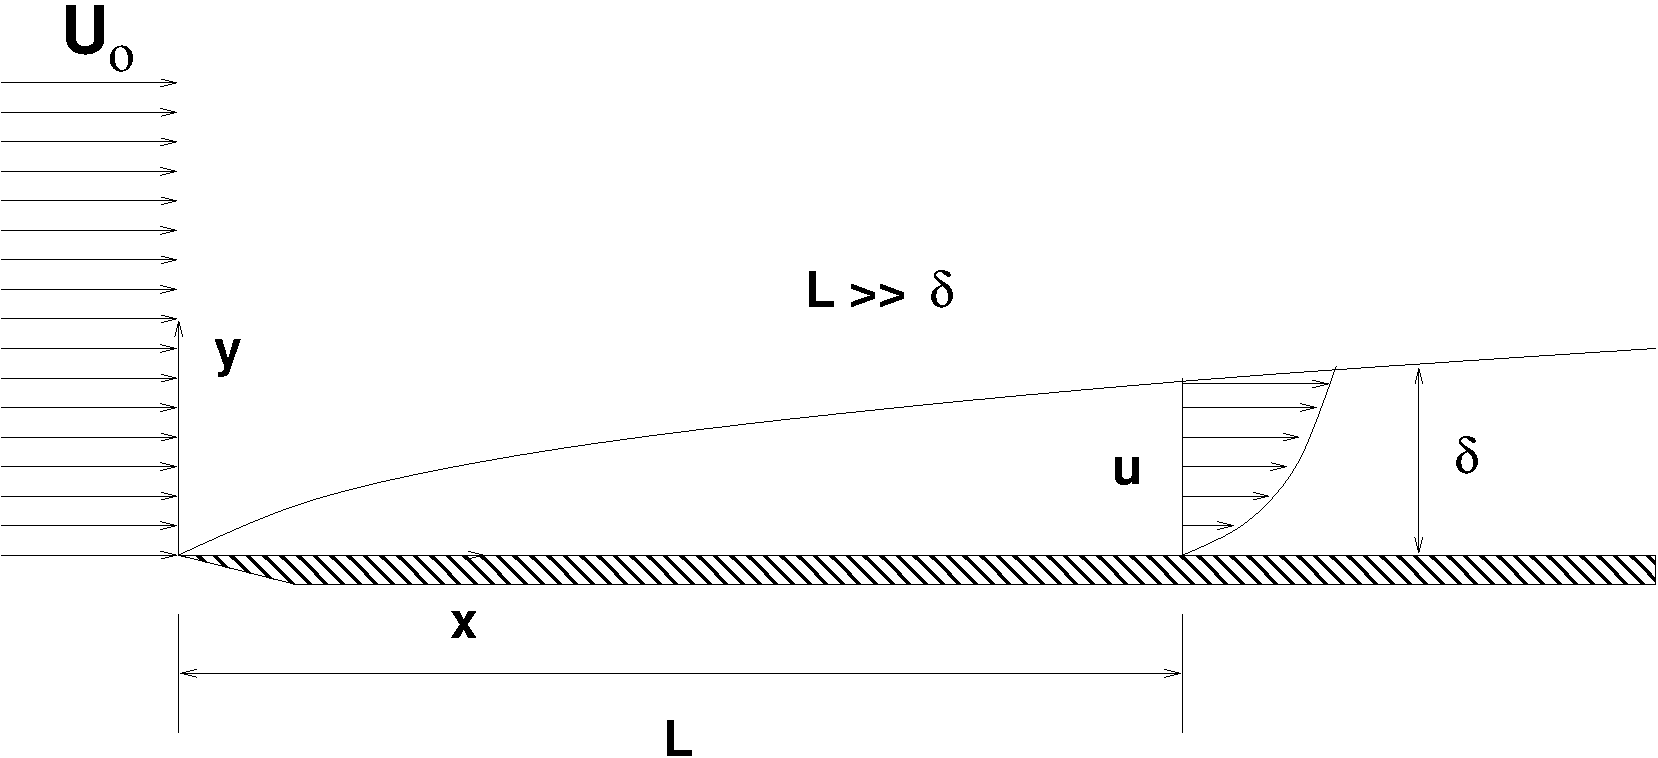
\includegraphics[width=\textwidth]{./figuras/camada-limite.pdf}

\end{frame}

\end{document}




\begin{frame}{}
\end{frame}

\begin{itemize}
\end{itemize}
